% $File: report.tex
% $Date: Fri May 10 23:58:01 2013 +0800
% $Author: wyx <ppwwyyxxc@gmail.com>

\documentclass[11pt,a4paper]{article}

\usepackage{fontspec,amsmath,amssymb,zhspacing,verbatim,minted,listings}
\usepackage{titlesec, titletoc}
\usepackage[hyperfootnotes=false,colorlinks,linkcolor=blue,anchorcolor=blue,citecolor=blue]{hyperref}
\usepackage[sorting=none]{biblatex}
%\usepackage[dvips]{graphicx}
\usepackage{subfigure}
\usepackage{indentfirst}
\usepackage{float}			% don't automatically change location of figure [H]
\usepackage{chngpage}		% use \changetext to change page size
\usepackage{caption}\captionsetup{hypcap=true}  % ref to jump to object instead of caption
\newfontfamily\zhfont[BoldFont=SimHei,ItalicFont=KaiTi_GB2312]{SimSun}
\lstset{keywordstyle=\color{blue!70}, commentstyle=\color{red!50!green!50!blue!50},frame=shadowbox,rulesepcolor=\color{red!20!green!20!blue!20},
basicstyle=\footnotesize\ttfamily}
\zhspacing
\setlength{\parindent}{2em}

%use cell in tabular
\newcommand{\tabincell}[2]{\begin{tabular}{@{}#1@{}}#2\end{tabular}}

%thick shline
\newlength\savewidth
\newcommand\shline{\noalign{\global\savewidth\arrayrulewidth\global\arrayrulewidth 1pt}
                   \hline
                   \noalign{\global\arrayrulewidth\savewidth}}


\renewcommand{\abstractname}{摘要}
\renewcommand{\contentsname}{目录}
\renewcommand{\tablename}{表}
\renewcommand{\figurename}{图}
\defbibheading{bibliography}{\section{References}}
\bibliography{refs.bib}
\newcommand{\figref}[1]{\hyperref[fig:#1]{图\ref*{fig:#1}}}
\newcommand{\secref}[1]{\hyperref[sec:#1]{\ref*{sec:#1}节}}
\newcommand{\tabref}[1]{\hyperref[tab:#1]{表\ref*{tab:#1}}}

% math function
\let\Oldsum\sum
\renewcommand{\sum}{\displaystyle\Oldsum}
\let\Oldprod\prod
\renewcommand{\prod}{\displaystyle\Oldprod}


% $File: mint-defs.tex
% $Date: Fri Jan 06 14:25:30 2012 +0800
% $Author: wyx <ppwwyyxxc@gmail.com>


% \inputmintedConfigured[additional minted options]{lang}{file path}{
\newcommand{\inputmintedConfigured}[3][]{\inputminted[fontsize=\footnotesize,
	label=#3,linenos,frame=lines,framesep=0.8em,tabsize=4,#1]{#2}{#3}}

% \phpsrc[additional minted options]{file path}: show highlighted php source
\newcommand{\phpsrc}[2][]{\inputmintedConfigured[#1]{php}{#2}}
% \phpsrcpart[additional minted options]{file path}{first line}{last line}: show part of highlighted php source
\newcommand{\phpsrcpart}[4][]{\phpsrc[firstline=#3,firstnumber=#3,lastline=#4,#1]{#2}}
% \phpsrceg{example id}
\newcommand{\phpeg}[1]{\inputminted[startinline,
	firstline=2,lastline=2]{php}{res/php-src-eg/#1.php}}

\newcommand{\txtsrc}[2][]{\inputmintedConfigured[#1]{text}{#2}}
\newcommand{\txtsrcpart}[4][]{\txtsrc[firstline=#3,firstnumber=#3,lastline=#4,#1]{#2}}

\newcommand{\pysrc}[2][]{\inputmintedConfigured[#1]{py}{#2}}
\newcommand{\pysrcpart}[4][]{\pysrc[firstline=#3,firstnumber=#3,lastline=#4,#1]{#2}}

\newcommand{\confsrc}[2][]{\inputmintedConfigured[#1]{squidconf}{#2}}
\newcommand{\confsrcpart}[4][]{\confsrc[firstline=#3,firstnumber=#3,lastline=#4,#1]{#2}}

\newcommand{\cppsrc}[2][]{\inputmintedConfigured[#1]{cpp}{#2}}
\newcommand{\cppsrcpart}[4][]{\cppsrc[firstline=#3,firstnumber=#3,lastline=#4,#1]{#2}}


\title{EXAMPLE}
\author{吴育昕\\(清华大学计算机系~北京~100084~ppwwyyxxc@gmail.com)}
\date{January, 2012}

\begin{document}
\changetext{}{2.2cm}{-1.1cm}{-1.1cm}{}
\setlength{\headheight}{15.2pt}

%\begin{abstract}

	%{\bf 关键词}
%\end{abstract}

% File: title.tex
% Date: Sun Aug 26 17:12:29 2012 +0800
% Author: Yuxin Wu <ppwwyyxxc@gmail.com>

\newcommand{\HUGE}{\fontsize{29pt}{29pt}\selectfont} 
\renewcommand{\today}{\number\year 年 \number\month 月 \number\day 日}
\begin{titlepage} 

% 首行的位置往上调整。但vspace前面需要有东西才会起效。

\phantom{Start!}

\vspace{-1.7cm} 

\begin{flushleft}

\emph{\Large 清华大学计算机系}\\[0.2cm]

\emph{\Large 并行程序设计}\\[4.2cm] 

% Title

%{ \Large \bfseries 程序设计作业一}\\[0.4cm]


{ \Huge \bfseries Mandelbrot Set}\\[0.4cm]

%{ \Large \bfseries 实现报告} \\[0.4cm]

\end{flushleft}

  

 

\vfill 

 

\begin{flushright}

{

%\setCJKmainfont{Adobe Kaiti Std}

% \pillar:使用一种统一的方法提高行高

\newcommand{\pillar}{ {\Huge \phantom{A}} }

\large

\begin{tabular}{lc}

\pillar 姓名 & 吴育昕\\\cline{2-2}

\pillar 学号 & 2011011271\\\cline{2-2}

\pillar 邮箱 & ppwwyyxxc@gmail.com \\\cline{2-2}

\pillar 时间 & 2012年8月 \\\cline{2-2}

%\pillar 报告日期 & 2012年3月22日 \\\cline{2-2}

\end{tabular}

} 

\end{flushright} 

\end{titlepage} 

\tableofcontents
\titleformat*{\section}{\centering\Large\bf}
% File: intro.tex
% Date: Sat May 11 00:00:07 2013 +0800
% Author: Yuxin Wu <ppwwyyxxc@gmail.com>
\section{Introduction}

\begin{enumerate}
	\item 编译:
		程序共有四个版本,分别为串行,MPI,OpenMP,pthread.需通过改变环境变量\verb|DEFINES|分别编译.源码中提供了一个脚本\verb|make_all_version|可以一次性编译出四个可执行文件.
		编译并行版本的环境变量分别为\verb|DEFINES=-DUSE_OMP, -DUSE_MPI, -DUSE_PTHREAD|,单独编译出的可执行文件为\verb|main|
\begin{lstlisting}
$ ./make_all_version
make seq verson ...
done
make omp version ...
done
make pthread version ...
done
make mpi version ...
done
$ DEFINES=-DUSE_OMP make
mkdir: created directory ‘obj’
[dep] ./calculate.cc ...
[dep] ./main.cc ...
[dep] ./Xoutput.cc ...
[dep] ./png_writer.cc ...
[cc] calculate.cc ...
[cc] Xoutput.cc ...
[cc] main.cc ...
[cc] png_writer.cc ...
Linking ...
$
\end{lstlisting}

\item 命令行参数:
	\begin{lstlisting}[basicstyle=\scriptsize\ttfamily]
$ ./main
Options:
  --nproc=NUM, -n      number of threads(pthread only). number of CPUs by default
  --size=SIZE, -s      size of picture. SIZE is of format `<width>x<height>'
                       eg. `800x800' (default),
  --domain=DOMAIN, -d  plotting domain. DOMAIN is of format
                       `<xmin>,<ymin>,<width>,<height>', where x and y are
                       the coordinates of left-bottom corner.
                       eg. `-2,-2,4,4` (default).
  --iter=NUM, -i       set max number of iteration of function. 1000 by default.
  --png=FILENAME, -p   save image to png file.
  --X, -x                              use X to show image. can move and zoom image.
  --help, -h           show this help and quit
\end{lstlisting}
程序支持如下的命令行参数:
\begin{description}
	\item \verb|--nproc=NUM|指定pthread使用的线程数量,对其他多线程模式无效.
	\item \verb|--size=SIZE|指定生成图片的大小.
	\item \verb|--domain=DOMAIN|指定绘图区域的坐标.
	\item \verb|--iter=NUM|指定计算时的迭代次数.
	\item \verb|--png=FILE|将结果输出到png文件中.
	\item \verb|--X|将图片用Xlib显示.
	\item \verb|--help|输出帮助信息.
\end{description}


\item 测试运行:
\begin{lstlisting}
$ ./omp -s 2000x2000
0.206523 seconds elapsed
$ ./pthread -s 2000x2000
0.199212 seconds elapsed
$ mpirun -n 4 ./mpi  -s 2000x2000
0.254203 seconds elapsed
$ ./seq -s 2000x2000
0.653799 seconds elapsed
$
\end{lstlisting}

\item 界面展示:
	\begin{lstlisting}
	$ ./pthread -x
	0.035687 seconds elapsed
	$
	\end{lstlisting}
	在X窗口中,可使用方向键移动屏幕,用``=''/``-''进行放大/缩小(由于精度限制,只能放大约$ 10^{15}$倍),用鼠标左右键改变区域中心再放大/缩小,s让程序从\verb|stdin|接收文件名并截图保存,
	c键从\verb|stdin|接受新的迭代次数取值,以观察同一位置在不同迭代次数下的不同图形.ESC键退出.

	窗口左上角显示的是窗口左下角坐标以及窗口在$ x,y$方向上跨越的坐标系上的长度.

	\begin{figure}[H]
      \begin{minipage}[b]{0.46\linewidth}
		\centering
		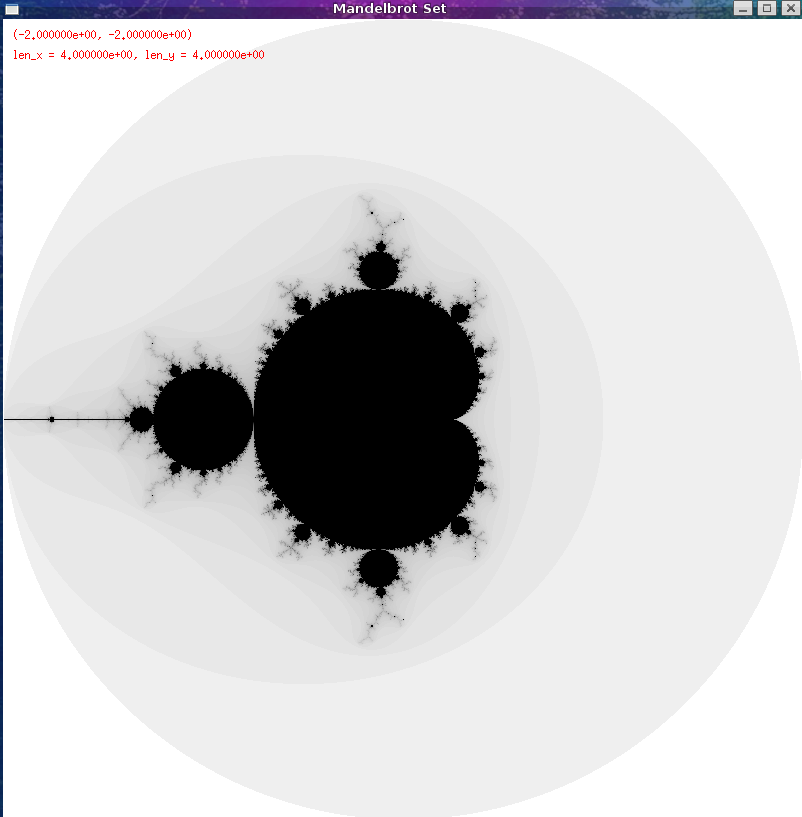
\includegraphics[scale=0.3]{res/show.png}
      \end{minipage}
      \begin{minipage}[b]{0.46\linewidth}
		\centering
		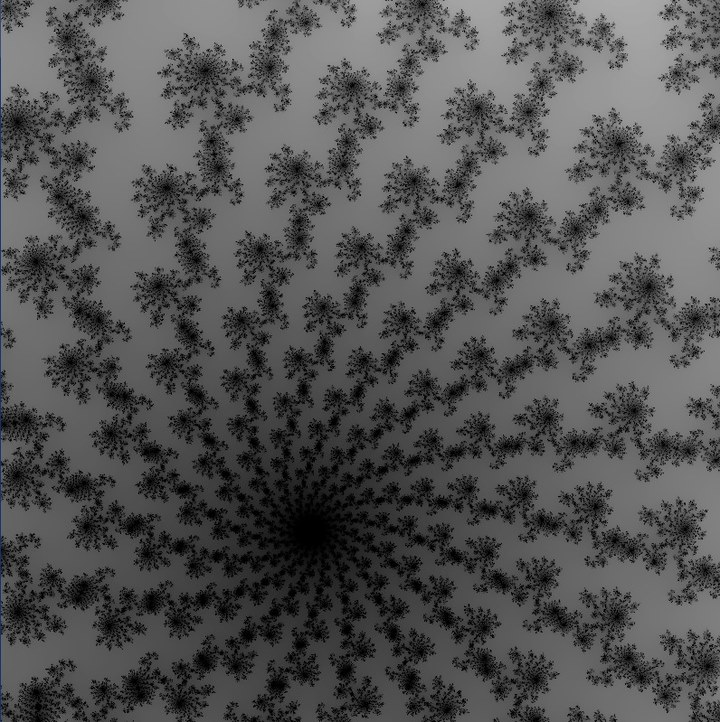
\includegraphics[scale=0.3]{res/showmore.jpg}
      \end{minipage}
	\end{figure}




\end{enumerate}

% File: theory.tex
% Date: Sat May 11 00:00:16 2013 +0800
% Author: Yuxin Wu <ppwwyyxxc@gmail.com>
\section{Algorithms}
\label{sec:algorithms}

{\bf 定义:}复平面上使得数列$ \{z_n\}: z_0 = 0; z_{n+1} = z_n^2 + c$收敛的全体复数c的集合称为Mandelbrot Set.

{\bf 定理:}$ \{z_n\}: z_0 = 0; z_{n+1} = z_n^2 + c $ 中有$ z_k $满足$ |z_k| > 2$,则$ \{ z_n\}$必发散.

{\bf 证明:}

首先可以看出,必存在$ z_k$满足$ |z_k| \ge |c|$且$ |z_k| > 2$. 当$ |c| \le 2$时显然存在,因为存在$ |z_k| > 2$.
当$ |c| > 2$时,$ |z_1| = |c| \ge |c|$满足条件.

于是,选取一个$ z_k$,满足$ |z_k| \ge |c|, |z_k| > 2$,那么一定$ \exists t > 0, |z_k| > 2 + t.$

我们可以得到如下的不等式:
\[ |z_{k+1}| = |z_k^2 + c| \ge |z_k^2| - |c| \ge |z_k^2| - |z_k| = (|z_k| - 1)|z_k| > (1 + t)|z_k| \]

迭代下去,有
\[ |z_{k+2}| = |z_{k+1}^2 + c| \ge |z_{k+1}^2| - |c| \ge |z_{k+1}^2| - |z_{k+1}| > (1+t)|z_{k+1}| > (1+t)^2|z_k|\]

$ \cdots \cdots$

于是,$ |z_{k+n}| > (1+t)^n|z_k|.$由于$ 1 + t > 1, $显然数列发散. 得证.
\\

由上述定理,计算一点$ c = c_r + c_ii$是否在Mandelbrot Set中,在迭代时一旦发现超出复平面上半径为2的圆,就可直接退出循环,大幅减少迭代时间.算法代码如下:
\cppsrcpart{res/src/calculate.cc}{40}{51}

利用类似手段,还可以得到一个结论:若$ |c| < \dfrac{1}{4}, $则数列必发散.
经实验,这个结论由于只对小范围数据有效,因此添加到程序中后(注释掉的代码)大多数情形下会影响程序效率.

% File: design.tex
% Date: Sun Aug 26 17:01:13 2012 +0800
% Author: Yuxin Wu <ppwwyyxxc@gmail.com>
\section{Design}
	程序通过编译选项\verb|-DUSE_MPI, -DUSE_OMP, -DUSE_PTHREAD|指定使用的多线程库,通过命令行参数指定算法迭代深度,绘图范围,图片大小等信息.
	初始化完毕后,程序调用\verb|MPI_Wtime()|计时,对指定区域计算,计算结束后将图像数据存放在\verb|short* img|中,输出所耗时间,如有必要则进行图形渲染,随后退出.

	当定义了\verb|USE_OMP|宏时,程序调用\verb|cal_rectangle_omp()|函数进行计算,函数中循环体前有\verb|#pragma omp parallel for schedule(dynamic)|一行,
对下方的for循环自动进行了动态多线程任务调度.
	
	当定义了\verb|USE_PTHREAD|宏时,程序调用\verb|cal_rectangle_pth()|函数.
	函数创建\verb|nproc|个线程,每个线程每次领取区域中十列数据的计算任务,并使用一个mutex用于记录当前未领的任务.
	
	当定义了\verb|USE_MPI|宏时,程序调用\verb|cal_rectangle_mpi()|函数.
	root进程只负责进行任务调度,将任务以100列资料为一个单位发送.各进程接收root发送的BEGIN信息以及任务的起始列数,便开始计算,计算完成后向root进程发送FINISH信息及计算数据.
	由于单个数据规模小,因此使用short进行储存以节省通信成本.

	数据计算完毕后,若需要输出png图片,则调用libpng库进行图片渲染.
	若需要实时显示,则初始化Xwindow, 将图片逐点绘制并开始接收键盘事件.
	接收到缩放,移动按键后对绘图参数进行处理,再调用计算函数重新绘制但不再计时,直至收到ESC按键,程序退出.

	在染色方面,经过多次尝试,设计出了一个关于迭代次数与最大迭代次数的函数代表各点的灰度,这个函数使得集合内的点为纯黑色,集合周围迭代次数较高的点为灰色,但与黑色无法充分接近,迭代次数少的点较白.
	这个配色函数可保证即使放大多倍,集合边界也十分明显,同时在最大迭代次数改变时常常能找到美丽的图案.

% File: analyse.tex
% Date: Fri Aug 31 00:50:20 2012 +0800
% Author: Yuxin Wu <ppwwyyxxc@gmail.com>
\section{Results and Analysis}
各参数对程序运行时间的影响:

\begin{enumerate}
	\item iter:\\
		程序在判断一个点是否属于集合中时,对一点迭代iter次,iter越高,所得图像越精确,集合边界越清晰,所花时间也越长.
		同时,由于程序配色函数比较特殊,iter取值的改变可能使得集合周围显示一些美妙图案.
		
		迭代次数极少时,集合边界非常圆滑,随着迭代次数增加,边界向内收缩.如\figref{shrink}


		\begin{figure}[H]
			\centering
			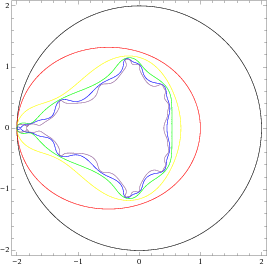
\includegraphics[scale=1]{res/shrink.png}
			\caption{\label{fig:shrink}}
		\end{figure}

\begin{lstlisting}
$ ./pthread -s 2000x2000 -i 1000
0.622379 seconds elapsed
$ ./pthread -s 2000x2000 -i 5000
2.880889 seconds elapsed
$ ./pthread -s 2000x2000 -i 8000
4.572143 seconds elapsed
$
\end{lstlisting}
从以上速度测试可以看出,iter增加到$ k$倍时,耗时略小于$ k$倍.这是因为对区域中的许多点,经过少量迭代就已经越界.


\item size:\\
\begin{lstlisting}
$ ./pthread -s 1000x1000
0.157242 seconds elapsed
$ ./pthread -s 2000x2000
0.622366 seconds elapsed
$ ./pthread -s 3000x3000
1.396862 seconds elapsed
$ ./pthread -s 4000x4000
2.478775 seconds elapsed
\end{lstlisting}
从数据可以看出,耗时的变化大约与点的个数成正比,耗时略少于$ k$倍,猜想是多线程的启动耗时,openmp,MPI也有类似情况.于是增大数据规模:


\begin{lstlisting}
$ ./pthread -s 10000x10000 -i 300
5.636299 seconds elapsed
$ ./pthread -s 10000x20000 -i 300
11.265757 seconds elapsed
$ ./pthread -s 20000x20000 -i 300
22.500245 seconds elapsed
$ ./pthread -s 20000x40000 -i 300
46.199222 seconds elapsed
$ ./pthread -s 30000x40000 -i 300
71.325897 seconds elapsed
\end{lstlisting}

数据规模变大后,线程启动耗时的影响渐渐可以忽略不计,此时可以看出,数据规模变为$ k$倍时,程序耗时略多于$ k$倍,这应当是线程间锁定/进程间通信耗时的结果.

\item domain:\\
	由于区域各点所执行的迭代次数不同,改变区域可能大幅改变程序效率.

\begin{lstlisting}
$ ./pthread -d -5,-5,2,2
0.008872 seconds elapsed
$ ./pthread -d -0.2,-0.2,0.1,0.1   
0.974035 seconds elapsed
\end{lstlisting}

\item nproc:\\
	使用pthread加速时,通过命令行参数改变nproc:
\begin{lstlisting}
$ ./pthread -n 2 -s 5000x5000
7.524309 seconds elapsed
$ ./pthread -n 4 -s 5000x5000                                                                                                                                                                                                                  
3.761441 seconds elapsed
$ ./pthread -n 8 -s 5000x5000
1.882019 seconds elapsed
$ ./pthread -n 16 -s 5000x5000
1.894062 seconds elapsed
$ ./pthread -n 32 -s 5000x5000
1.935740 seconds elapsed
\end{lstlisting}
	使用MPI加速时,利用mpirun改变nproc:
\begin{lstlisting}
$ mpirun -n 2 ./mpi -s 5000x5000
15.010539 seconds elapsed
$ mpirun -n 4 ./mpi -s 5000x5000
5.037870 seconds elapsed
$ mpirun -n 6 ./mpi -s 5000x5000
3.273679 seconds elapsed
$ mpirun -n 8 ./mpi -s 5000x5000
2.186701 seconds elapsed
$ mpirun -n 9 ./mpi -s 5000x5000
2.895381 seconds elapsed
$ mpirun -n 16 ./mpi -s 5000x5000
3.586846 seconds elapsed
\end{lstlisting}

\begin{lstlisting}
$ ./omp -s 5000x5000
1.887277 seconds elapsed
\end{lstlisting}


\begin{figure}[H]
\centering
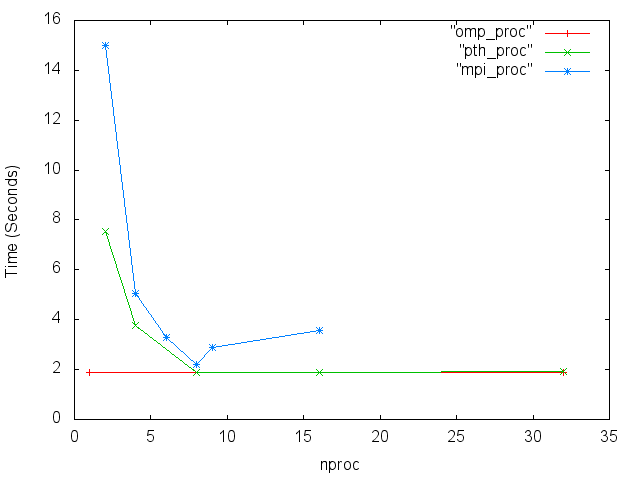
\includegraphics[scale=0.5]{res/chart.png}
\end{figure}

由以上数据(由清华大学FIT楼集群计算机生成)可以看出,对于pthread, 线程数等于处理器个数时最佳.对于MPI,由于此程序有一进程只负责管理任务,因此效率与进程数关系可能略有不同,无法与pthread进行直接比较.但从数据来看仍是8个进程时效率最高.
而且由于MPI的进程通信及初始化更为复杂,因此进程数更高时效率会明显下降.
OpenMP由于设置成自动分配,无法改变线程数,但其效率很高.

对于更大规模的数据,只能使用MPI进行多节点测试,测试数据如下.

\begin{table}[h]
	\centering
	\begin{tabular}{c|c}
		\hline
	nproc & time \\\hline
	24 & 373.262603 \\
	36 &281.326281 \\
	48 &203.073978\\
	60 &169.850154\\
	72 &157.953276 \\\hline
\end{tabular}
\end{table}

\begin{figure}[H]
	\centering
	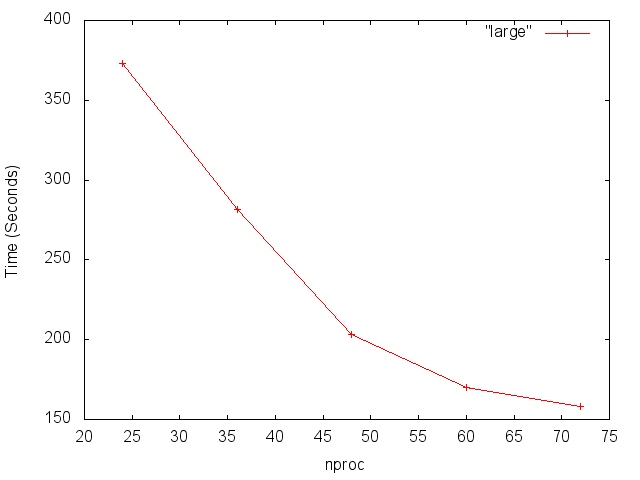
\includegraphics[scale=0.6]{res/large.png}
\end{figure}
测试参数: -s 30000x30000 -i 20000

\end{enumerate}

% File: exp.tex
% Date: Sun Aug 26 21:02:38 2012 +0800
% Author: Yuxin Wu <ppwwyyxxc@gmail.com>
\section{Experience}
	这次使用三种并行库分别进行多线程程序设计,让我有很大进步.
	首先是对于三种并行库都有了更深入的了解.OpenMP程序实现上最容易,但对算法有较大要求,对多线程需要共享信息的情形会难以实现.
Pthread是一个方便的多线程库,编程上难度不大,同时也有\verb|mutex_lock|机制使线程间可以进行信息交流.
MPI由于是多进程的,因此无法共享内存,需要另外使用消息机制来管理通信,因此在实现上较为复杂,需要在原始版本上增添不少代码,效率也不高.
但这也使得MPI程序可以在多个机器上共同运行,适合计算更加巨型的任务.

	上次作业我使用gtkmm创建GUI,这次便改用了Xlib. 相比之下Xlib操作简单,但功能较少.
	尤其是在event处理上只能采用时刻不停接收的方法.如果有多个事件短时间内发生,会一个接一个处理,对性能十分不利.
	例如对于窗口的拉伸操作,就会一次性触发大量\verb|ConfigureNotify|事件,造成程序多次刷新.
	同时,由于多进程/多线程操作内部实现复杂,因此与较复杂的图形库共用时也许会有不可预见的后果,而Xlib的简单结构较易于掌控.

	另外,这次作业生成的Mandelbrot Set,是一个经典的分形图形,将其放大可以找到大量的美丽图片,使我们在完成作业的同时深刻感受到了数学之美.
	

\printbibliography
% File: appendix.tex
% Date: Fri May 10 23:19:33 2013 +0800
% Author: Yuxin Wu <ppwwyyxxc@gmail.com>
%\section{Source Code}
%\txtsrc{res/src/main.cc}

%\txtsrc{res/src/include/calculate.h}

%\txtsrc{res/src/include/Xoutput.h}

%\txtsrc{res/src/include/pngwriter.h}

%\txtsrc{res/src/calculate.cc}

%\txtsrc{res/src/Xoutput.cc}

%\txtsrc{res/src/pngwriter.cc}


\end{document}

